%%%%%%%%%%%%%%教案头%%%%%%%%%%%%%%%%%%%%%%%%%%%%%%%
\mode<article>{

\begin{longtable}{|m{20mm}|m{20mm}|m{20mm}|m{20mm}|m{20mm}|m{28mm}|}
\caption*{\huge 教案头}\\
\hline
\endfirsthead
\multicolumn{6}{l}{(续表)}\\
\hline
\endhead
\hline
\multicolumn{6}{l}{\itshape 接下一页表格.......}\\ [2ex]
\endfoot
\hline
\endlastfoot
\centering{授课单元}&\multicolumn{3}{m{60mm}|}{\centering 2.6.4二阶系统的动态响应}&\centering{授课日期}&2014年04月14日 \\
\hline
\centering 授课地点 & \multicolumn{3}{m{60mm}|}{B6-204}&\centering 授课学时 & 2 \\
\hline
& \multicolumn{2}{m{40mm}|}{能力目标} & \multicolumn{2}{m{40mm}|}{知识目标}&素质目标 \\
\cline{2-6}
\centering 教学目标&\multicolumn{2}{m{40mm}|}{\begin{enumerate}
\item 能够分析二阶系统的动态响应
\item 能够计算二阶系统的性能指标
\end{enumerate} }&\multicolumn{2}{m{40mm}|}{\begin{enumerate}
\item 了解二阶系统的数学模型
\item 掌握二阶系统的响应分析
\end{enumerate}} & {\qquad}\\
\hline
\centering 能力训练任务或案例 &\multicolumn{5}{m{108mm}|}{ }\\
\hline
\centering 教学重点 & \multicolumn{5}{m{108mm}|}{\begin{enumerate}
\item 二阶系统的动态响应
\end{enumerate}}\\
\hline
\centering 教学难点与解决办法 &\multicolumn{5}{m{108mm}|}{\begin{enumerate}
\item 难点:二阶系统的动态响应分析
\item 解决方法:用实例进行分析讲解
\end{enumerate}}\\
\hline
\centering 德育内容 &\multicolumn{5}{m{108mm}|}{无}\\
\hline
 &教材 & \multicolumn{4}{m{88mm}|}{计算机控制原理与应用}\\
\cline{2-6}& 教学资源 &\multicolumn{4}{m{88mm}|}{PPT}\\
\cline{2-6}\centering 使用的教学材料& 主要教学仪器设备和工具等 &\multicolumn{4}{m{88mm}|}{投影机、MATLAB}\\
\cline{2-6}& 主要耗材 &\multicolumn{4}{m{88mm}|}{无}\\
\hline
\centering 教学模式 &\multicolumn{2}{m{40mm}|}{知识讲授}&\centering 教学手段 &\multicolumn{2}{m{48mm}|}{多媒体教学}\\
\hline
\centering 学生成果与过程考核方式 &\multicolumn{5}{m{108mm}|}{无}
\end{longtable}
\clearpage

%%%%%%%%%%%%%%%教学实施过程%%%%%%%%%%%%%%%%%%%%%%%%%%%%
\begin{landscape}

\begin{longtable}{|m{10mm}|m{50mm}|m{50mm}|m{50mm}|m{15mm}|}
\caption*{\huge 教学组织与实施}\\
\hline
\endfirsthead
\multicolumn{5}{l}{\small 接上页}\\
\hline
\multicolumn{1}{|c|}{步骤}&\multicolumn{1}{c|}{教学内容}&\multicolumn{1}{c|}{教师活动}&\multicolumn{1}{c|}{学生活动}&\multicolumn{1}{c|}{时间}\\
\hline
\endhead

\multicolumn{5}{r}{\small 接下页}\\
\endfoot
\hline
\endlastfoot
\multicolumn{1}{|c|}{步骤}&\multicolumn{1}{c|}{教学内容}&\multicolumn{1}{c|}{教师活动}&\multicolumn{1}{c|}{学生活动}&\multicolumn{1}{c|}{时间}\\\hline
讲解&\begin{enumerate}
\item 二阶系统的数学模型
\end{enumerate} &\begin{enumerate}
\item 讲解分析二阶系统的数学模型
\end{enumerate} &\begin{enumerate}
\item 学生倾听并记录
\end{enumerate} &15 \\\hline
讲解&\begin{enumerate}
\item 二阶系统的单位阶跃响应
\end{enumerate}
 &\begin{enumerate}
\item 通过数学分析和图示讲解二阶系统的单位阶跃响应
\end{enumerate} &\begin{enumerate}
\item 学生倾听并记录
\end{enumerate} &30 \\\hline
讲解&\begin{enumerate}
\item 典型二阶系统的动态性能指标
\end{enumerate}
&\begin{enumerate}
\item 讲解二阶系统的动态性能指标
\end{enumerate} &\begin{enumerate}
\item 学生倾听并记录
\end{enumerate} &20 \\\hline
讲解&\begin{enumerate}
\item 二阶系统的单位脉冲响应
\end{enumerate}
 &\begin{enumerate}
\item 讲解阶系统的单位阶跃响应分析
\end{enumerate} &\begin{enumerate}
\item 学生记录笔记
\end{enumerate} &20 \\\hline
总结&
\begin{enumerate}
\item 二阶系统的动态响应
\end{enumerate}
 &\begin{enumerate}
\item 总结二阶系统的动态响应
\end{enumerate} &\begin{enumerate}
\item 学生记录笔记
\end{enumerate} &5 \\\hline
\centering 本次课总结(评价)&总结本课程内容 &进行知识总结 &学生倾听 &5 \\\hline
\centering 学生学习笔记或工单等检查情况&\multicolumn{4}{m{165mm}|}{\quad}\\\hline
\centering 课后作业&\multicolumn{4}{m{165mm}|}{2-19,2-20,2-21}\\\hline
\centering 教学体会&\multicolumn{4}{m{165mm}|}{\quad}\\
\end{longtable}

\end{landscape}
\clearpage
%%%%%%%%%%%%%%%%%%%%板书设计%%%%%%%%%%%%%%%%%%%%%%%%%%
\begin{center}
{\huge 板书设计}
\end{center}
}
\mode<presentation>{ \section{控制系统的时域分析}
 \subsection{二阶系统的动态响应}}
 \begin{frame}{二阶系统的数学模型}
 \begin{block}{}
 \begin{itemize}
 \item<+-> RLC网络的二阶微分方程:
 \[\frac{d^2c(t)}{dt^2}+\frac{R}{L}\frac{dc(t)}{dt}+\frac{1}{LC}c(t)=\frac{1}{LC}r(t)\]
 \item<+-> 典型形式为:
 \[\frac{d^2c(t)}{dt^2}+2\zeta\omega_n\frac{dc(t)}{dt}+\omega_n^2=\omega_n^2r(t)\]
 \end{itemize}
 \end{block}
 \end{frame}
 
 \begin{frame}
 \begin{block}{}
 \begin{itemize}
 \item<+-> 其中:
 \[\omega_n=\frac{1}{\sqrt{LC}}\]
 \[2\zeta\omega_n=\frac{R}{L}\]
 \[\zeta=\frac{R}{2}\sqrt{\frac{C}{L}}\]
\end{itemize}  
\end{block}
\end{frame}

\begin{frame}
\begin{block}{}
\begin{itemize}
\item<+-> 进行拉氏变换得:
\[s^2C(s)+2\zeta\omega_nsC(s)+\omega_n^2C(s)=\omega_n^2R(s)\]
\item<+-> 系统开环传递函数为:
\[G_o(s)=\frac{C(s)}{E(s)}=\frac{\omega^2_n}{s(s+2\zeta\omega_n)}\]
\end{itemize}
\end{block}
\end{frame}
\begin{frame}
\begin{block}{}
\begin{itemize}
\item<+-> 系统闭环传递函数为:
\[\Phi(s)=\frac{C(s)}{R(s)}=\frac{\omega_n^2}{s^2+2\zeta\omega_ns+\omega_n^2}\]
\item<+-> 系统特征方程为:
\[s^2+2\zeta\omega_ns+\omega_n^2=0\]
\end{itemize}
\end{block}
\end{frame}
\begin{frame}
\uncover<+->{\begin{block}{}
特征根为:
\[s_{1,2}=-\zeta\omega_n\pm\omega_n\sqrt{\zeta^2-1}\]
\end{block}}
\uncover<+->{\begin{block}{}
系统的特征取决于$\zeta$和$\omega_n$两个参数
\end{block}}
\end{frame}

\begin{frame}{二阶系统的单位阶跃响应}
\begin{block}{}
\begin{itemize}
\item<+-> 单位阶跃函数的拉氏变换为:
\[R(s)=\frac{1}{s}\]
\item<+-> 系统输入的拉氏变换为:
\[C(s)=\Phi(s)R(s)=\frac{\omega_n^2}{s^2+2\zeta\omega_ns+\omega_n^2}\cdot\frac{1}{s}\]
\end{itemize}
\end{block}
\end{frame}
\begin{frame}
\begin{block}{当$\zeta=0$时}
\begin{itemize}
\item<+-> 则:
\[C(s)=\frac{\omega_n^2}{s^2+\omega_n^2}\cdot\frac{1}{s}\]
\item<+-> 展开得:
\[C(s)=\frac{\omega_n^2}{s(s^2+\omega_n^2)}=\frac{1}{s}-\frac{s}{s^2+\omega_n^2}\]
\end{itemize}
\end{block}
\end{frame}
\begin{frame}
\begin{block}{}
\begin{itemize}
\item<+-> 拉氏逆变换得:
\[c(t)=1-\cos\omega_nt\]
\item<+-> 系统响应曲线:

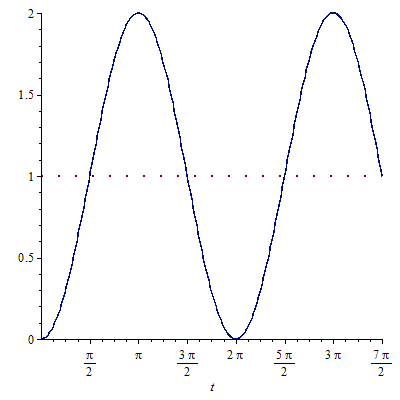
\includegraphics[scale=0.25]{wuzuni.png}
\end{itemize}
\end{block}
\end{frame}
\begin{frame}
\begin{block}{当$0<\zeta<1$时}
\begin{itemize}
\item<+-> 系统特征方程根为:
\[s_1=-\zeta\omega_n+j\omega_n\sqrt{1-\zeta^2}=-\zeta\omega_n+j\omega_d\]
\[s_2=-\zeta\omega_n-j\omega_n\sqrt{1-\zeta^2}=-\zeta\omega_n-j\omega_d\]
\end{itemize}
其中:$\omega_d=\omega_n\sqrt{1-\zeta^2}$
\end{block}
\end{frame}
\begin{frame}
\begin{block}{}
\begin{itemize}
\item<+-> 特征方程可写为:
\begin{eqnarray*}
s^2+2\zeta\omega_ns+\omega_n^2\\
=(s+\zeta\omega_n-j\omega_d)(s+\zeta\omega_n+j\omega_d)
\end{eqnarray*}
\end{itemize}
\end{block}
\end{frame}
\begin{frame}
\begin{block}{}
系统输出$C(s)$为:
\begin{eqnarray*}
C(s)=\Phi(s)R(s)=\frac{\omega_n^2}{s^2+2\zeta\omega_ns+\omega_n^2}\frac{1}{s}\\
=\frac{1}{s}-\frac{s+\zeta\omega_n}{(s+\zeta\omega_n)^2+\omega_d^2}-\frac{\zeta\omega_n}{(s+\zeta\omega_n)^2+\omega_d^2}
\end{eqnarray*}
\end{block}
\end{frame}
\begin{frame}
\begin{block}{}
\begin{itemize}
\item<+-> 拉氏逆变换为:
\begin{eqnarray*}
c(t)=L^{-1}[C(s)]\\
=1-e^{-\zeta\omega_nt}\frac{1}{\sqrt{1-\zeta^2}}\sin(\omega_dt+\varphi),t\geq 0
\end{eqnarray*}
\end{itemize}
\end{block}
\end{frame}
\begin{frame}
\begin{block}{当$\zeta=1$时}
\begin{itemize}
\item<+-> 系统的特征方程为:
\[s^2+2\zeta\omega_ns+\omega_n^2=s^2+2\omega_n+\omega_n^2=(s+\omega_n)^2\]
\item<+-> 系统输出为:
\[C(s)=\Phi(s)R(s)=\frac{\omega_n^2}{(s+\omega_n)^2}\cdot\frac{1}{s}\]
\end{itemize}
\end{block}
\end{frame}
\begin{frame}
\begin{block}{}
\begin{itemize}
\item<+-> 展开得:
\begin{eqnarray*}
C(s)=\frac{\omega_n^2}{s(s+\omega_n)^2}\\
=\frac{1}{s}-\frac{1}{s+\omega_n}-\frac{\omega_n}{(s+\omega_n)^2}
\end{eqnarray*} 
\item<+-> 拉氏逆变换得:
\[c(t)=1-e^{-\omega_nt}-e^{\omega_nt}\omega_nt,t\geq 0\]
\end{itemize}
\end{block}
\end{frame}
\begin{frame}{典型二阶系统的动态性能指标}
\begin{block}{}
\begin{itemize}
\item<+-> 延迟时间$t_d$:
\[t_d=\frac{0.7\zeta+1}{\omega_n}\]
\item<+-> 上升时间$t_r$:
\[t_r=\frac{1}{\omega_n}\arctan(1-\frac{\sqrt{1-\zeta^2}}{\zeta}=\frac{\pi-\varphi}{\omega_n}\]
\end{itemize}
\end{block}
\end{frame}
\begin{frame}
\begin{block}{}
\begin{itemize}
\item<+-> 峰值时间$t_p$:
\[t_p=\frac{\pi}{\omega_d}=\frac{\pi}{\omega_n\sqrt{1-\zeta^2}}\]
\item<+-> 最大超调量$M_p$:
\[M_p\%=e^{-\frac{\zeta\pi}{\sqrt{1-\zeta^2}}}\%\]
\end{itemize}
\end{block}
\end{frame}
\begin{frame}
\begin{block}{}
\begin{itemize}
\item<+-> 5\%调整时间:
\[t_s\approx\frac{1}{\zeta\omega_n}\ln(0.05\sqrt{1-\zeta^2})\]
\item<+-> 2\%调整时间:
\[t_s\approx\frac{1}{\zeta\omega_n}\ln(0.02\sqrt{1-\zeta^2})\]
\end{itemize}
\end{block}
\end{frame}
\endinput